\chapter{湖泊模式}
%\addcontentsline{toc}{chapter}{湖泊模式}
湖泊作为陆地表面一种特定形式的水体,对区域尺度的水热平衡过程及气候变化具有显著影响,其中大面积的湖泊对于局地的天气和气候可起到决定性作用。
为模拟湖泊的热力和动力过程,湖泊模式在上世纪80年代开始发展\citep{henderson1985new},
并逐渐形成针对不同湖泊的简易湖泊模式\citep{hostetler1993interactive,hostetler1994lake,hostetler1990simulation}。
此后,湖泊模式作为陆面过程模式的重要组成模块,其应用逐渐发展到针对全球湖泊的普适性模拟(e.g. \citet{bonan1995sensitivity,bonan1996land})。
\citet{zeng2002coupling}对当时已有的湖泊模式进行了改进,
使得湖泊模式的模拟效果得到显著提高,成为通用陆面模式CoLM中湖泊模型的早期版本(CoLM-lake)。
近几年来,随着湖泊模型的不断发展,CoLM-Lake逐渐纳入了新的针对湖泊方案的发展与改进,
并在2014年发布的新版CoLM中对湖泊模型进行了更新。本文将对新版CoLM-Lake的物理方案做一详细描述(图\ref{fig:湖泊系统垂直分层示意图})。
{
\begin{figure}[]
\centering
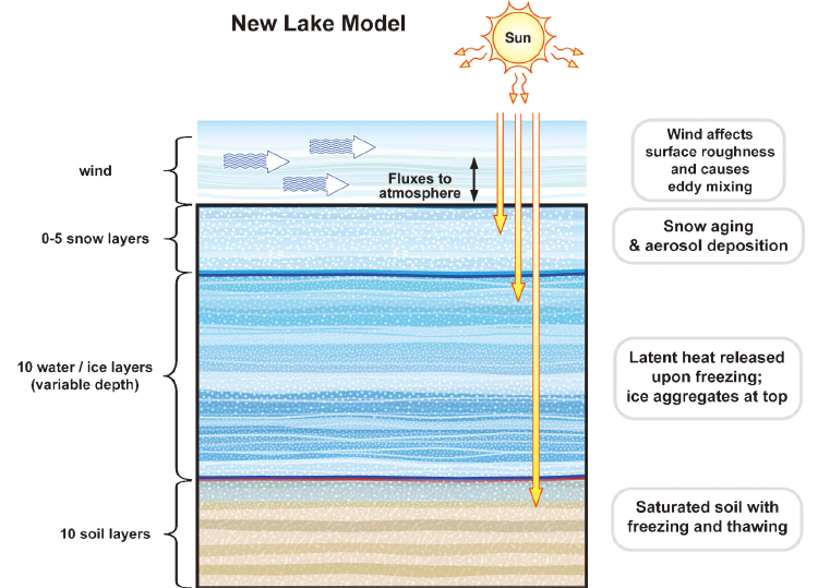
\includegraphics{Figures/湖泊模式/湖泊系统垂直分层示意图.png}
\caption{湖泊系统垂直分层示意图 \citep{subin2012improved}。}
\label{fig:湖泊系统垂直分层示意图}
\end{figure}
}

\section{湖泊模式结构}
湖泊模式由三部分组成:雪层、湖泊层和土壤层。湖泊层位于雪层和土壤层之间,
共分为10层,默认湖深$d$为50 m,每层湖泊的厚度$\Delta z_{lake,i}$从上到下分别为0.1, 1, 2, 3, 4, 5, 7, 7, 10.45, 10.45 m,
中心深度$z_{lake,i}$为每层湖泊的中间位置所在深度,分别为0.05, 0.6, 2.1, 4.6, 8.1, 12.6, 18.6, 25.6, 34.325, 44.775 m。
湖泊深度d亦可由地表参数数据集提供。当$d\neq50$m且$d\geq1$m时,第一层湖泊的厚度仍保持0.1 m,
其余层厚度按照上述分层厚度的比例进行分配。
当$d<1$m时,10层湖泊进行等分。在模式中,每层湖泊的质量固定不变,由液态水密度与每层湖泊的厚度确定,
湖泊状态变量由湖泊温度$T_{lake}$与冻结部分所占的质量比$I$来表征。雪层与土壤层的分层方式与 \ref{温度求解的数值格式} 节介绍的计算雪盖土壤温度时的分层方案相同
,物理方案遵从无植被覆盖下的土壤雪盖状态变量的计算方案来设定。
\section{降水与湖泊表面的相互作用}
降水到达湖泊表面可发生能量转移与相态变化等一系列过程。此过程可改变湖泊表面条件,尤其当降雪存在时,对于湖泊之上雪层的形成起到决定性作用。


首先,在进行湖泊过程计算之前,对湖泊表面的积雪厚度$z_{sno}$(m)与雪水当量$W_{sno}$(mm或$\rm kg/m^2$)进行更新:
\begin{equation}
Z_{sno}=Z_{sno}+\frac{p_{i} \Delta t}{\rho_{sno,new}}
\end{equation}
\begin{equation}
W_{sno}=W_{sno}+p_{i} \Delta t
\end{equation}
其中$p_i$表示固态降水率($\rm kg/m^2$/s),$\rho_{sno,new}$表示新降的干雪密度(kg/m3)(见章节  \ref{温度求解的数值格式})。
接下来,计算湖泊表面与降水的能量转移过程,并且当降水与湖泊表面的相态不同时,相态变化过程同时考虑。
此过程将根据更新后的积雪厚度,分为湖泊表层
\begin{enumerate}
    \item 未达到第一层雪的产生条件;
    \item 已达到第一层雪产生条件但之前无雪层;
    \item 之前已存在雪层,三种情况进行计算。
\end{enumerate}

\textbf {(1)未达到第一层雪产生条件(即$z_{sno}<0.01$且$snl=0$)}\\
此情形下,降水视为与第一层湖泊表面充分接触并立即发生能量转移,并且当降水与湖泊表层的相态不同时,相态变化过程同时发生。
此过程的演变由以下八个能量组份($\rm J/m^2$)决定:
\begin{align*}
a &= C_{pl} p_{l} \Delta t\left(T_{p}-T_{f}\right)   & \text{液态降水冷却到$T_f$释放的能量} \\
b &= L_f p_l \Delta t                                           & \text{液态降水凝结为固态释放的能量} \\
c &= C_{pi} \rho_{liq} \Delta z_{lake, 1} I_{1}\left(T_f-T_{lake, 1}\right)  & \text{第一层湖泊固态下加热到$T_f$吸收的能量} \\
d &= L_f \rho_{liq} \Delta z_{lake, 1} I_{1}         & \text{第一层湖泊固态下完全融化吸收的能量} \\
e &= C_{pi} p_i \Delta t\left(T_f -T_p\right)        & \text{固态降水加热到$T_f$吸收的能量} \\
f &= L_f p_i \Delta t                                           & \text{固态降水融化为液态吸收的能量} \\
g &= C_{pl} \rho_{liq} \Delta z_{lake, 1}\left(1-I_{1}\right)\left(T_{lake, 1}-T_f\right)  & \text{第一层湖泊液态下冷却到$T_f$释放的能量} \\
h &= L_f \rho_{liq} \Delta z_{lake, 1}\left(1-I_{1}\right)  & \text{第一层湖泊液态下完全冻结释放的能量}
\end{align*}
其中,$p_l$、$p_i$分别为液态与固态降水率($\rm kg/m^2$/s),$C_{pl}$、$C_{pi}$分别为液态水与固态水的比热容(J/kg/K),
$T_p$、$T_f$分别为雨水温度与液态水凝结温度(K),$\Delta t$表示时间积分步长(s),$L_f$表示液态水凝结潜热(J/kg),
$\rho_{liq}$表示液态水密度($\rm kg/m^3$),$T_{lake,1}$,$\Delta z_{lake,1}$,$I_1$分别为第一层湖泊的温度,
厚度与冻结部分所占的质量比。为表述清晰,此过程将按照第一层湖泊的不同相态分别考虑,计算如下:\\

A. 第一层湖泊完全冻结($I_1>0.999$)\\
此时,应有$T_{lake,1}<T_f$。若固态降水发生($T_p<T_f$),它将直接与湖泊表层达到一个平衡温度;
若液态降水发生($T_p>T_f$),相态变化过程将会同时触发,具体如下:

若表层湖泊不需发生相态变化足以使得液态降水到达表面后凝结为固态,即$a\le c-b$,则湖泊吸收的总能量为:
\begin{equation}
C_{pi} \rho_{liq} \Delta z_{lake,1} I_{1}\left(T_{lake, 1}^{(n+1)}-T_{\text {lake,1 }}^{(n)}\right)=a+b+C_{pi} p_{l} \Delta t\left(T_{f}-T_{\text {lake, }}^{(n+1)}\right)
\end{equation}
解出$T_{lake,1}^{\left(n+1\right)}$即为此时更新的第一层湖泊温度。
同时后续计算中,液态降水可视为固态降水,雪水当量与积雪厚度随之更新:
\begin{equation}
\begin{aligned}
W_{sno} &= W_{sno}+p_l \Delta t \\ 
z_{sno} &= z_{sno}+\frac{p_l \Delta t}{\rho_{sno,new}} \\ 
p_i &= p_i + p_l \\ 
p_l &= 0.0
\end{aligned}
\end{equation}


若表层湖泊将液态降水冷却到$T_f$后不足以冻结所有降水,即$c-b<a\le c$,
则第一层湖泊温度更新为$T_{lake,1}=T_f$。于是湖泊吸收的来自降水凝结的有效能量为$c-a$,
液态降水转为固态降水的量以及雪水当量和积雪厚度可更新为:
\begin{equation}
\begin{aligned}
W_{sno} &= W_{sno} + (c-a) / L_f \\ 
z_{sno} &= z_{sno} + \frac{c-a}{L_f \rho_{sno,new}} \\ 
p_i &= p_i + \frac{c-a}{L_f \Delta t} \\ 
p_l &= p_l - \frac{c-a}{L_f \Delta t}
\end{aligned}
\end{equation}
若表层湖泊需要部分融化才可将液态降水冷却到$T_f$而降水无需发生相态变化,即$c<a\le c+d$,
则第一层湖泊温度仍更新为$T_{lake,1}=T_f$。于是降水冷却用于融化湖泊的有效能量为$a-c$,
此时湖泊冻结部分所占的质量比更新为:
\begin{equation}
I_{1}=\frac{\rho_{liq} \Delta z_{lake, 1}-(a-c) / L_{f}}{\rho_{liq} \Delta z_{lake, 1}}
\end{equation}
若表层湖泊可被液态降水完全融化而降水无需发生相态变化,即$a>c+d$,则降水释放的总能量为:
\begin{equation}
C_{pl} p_{l} \Delta t\left(T_{p}-T_{lake, 1}^{(n+1)}\right)=c+d+C_{pl} \rho_{liq} \Delta z_{lake, 1}\left(T_{lake, 1}^{(n+1)}-T_{f}\right)
\end{equation}
解出$T_{lake,1}^{\left(n+1\right)}$即为此时更新的第一层湖泊温度,同时湖泊冻结部分质量比更新为$I_1=0.0$。


注意,经过以上情况讨论后,若发生液态降水冻结为固态降水,则雪水当量与积雪厚度将会增加。
此时若$z_{sno}\geq0.01$m,则第一层雪立即生成,且相应的状态变量设置为:
\begin{equation}
\begin{aligned}
    snl &= -1 \\ 
    \Delta z_{0} &= z_{sno} \\ 
    z_{0} &= -0.5 z_{sno} \\
    z_{h,-1} &= -\Delta z_{0} \\ 
    T_{0} &= T_{lake, 1} \\
    w_{ice, 0} &= W_{sno} \\
    w_{liq, 0} &= 0
\end{aligned}
\end{equation}

B. 第一层湖泊为冰水混合态($0.001\le I_1\le0.999$)\\
此时,应有$T_{lake,1}=T_f$。若液态降水发生($T_p>T_f$),
当液态降水可以将第一层湖泊中的冰全部融化时($a\geq d$),第一层湖泊的状态变量更新为:
\begin{equation}
T_{lake, 1}=\frac{C_{pl} p_{l} \Delta t T_{p}+C_{pl} \rho_{liq} \Delta z_{lake, 1} T_{f}-d}{C_{pl} \rho_{liq} \Delta z_{lake, 1}+C_{pl} p_{l} \Delta t}
\end{equation}
\begin{equation}
I_{1}=0.0
\end{equation}
否则,保持$T_{lake,1}=T_f$,用于湖泊中冰融化的能量为$a$,则湖泊冻结部分的质量比更新为:
\begin{equation}
I_{1}^{(n+1)}=\frac{\rho_{liq} \Delta z_{lake, 1} I_{1}^{(n)}-a / L_{f}}{\rho_{liq} \Delta z_{lake, 1}}
\end{equation}
同样地,若固态降水发生($T_p<T_f$),当固态降水可以将第一层湖泊中的水全部冻结时($e\geq h$),第一层湖泊的状态变量更新为:
\begin{equation}
T_{lake, 1}=\frac{C_{p i} p_{i} \Delta t T_{p}+C_{p i} \rho_{liq} \Delta z_{lake, 1} T_{f}+h}{C_{p i} \rho_{liq} \Delta z_{lake, 1}+C_{p i} p_{i} \Delta t}
\end{equation}
\begin{equation}
I_{1}=1.0
\end{equation}
否则,保持$T_{lake,1}=T_f$,用于湖泊中水冻结的能量为$e$,则湖泊冻结部分的质量比更新为:
\begin{equation}
I_{1}^{(n+1)}=\frac{\rho_{liq} \Delta z_{lake, 1} I_{1}^{(n)}+e / L_{f}}{\rho_{liq} \Delta z_{lake, 1}}
\end{equation}

C. 	第一层湖泊完全融化($I_1<0.001$)\\
此时,应有$T_{lake,1}>T_f$。若液态降水发生($T_p>T_f$),它将直接与湖泊表层达到一个平衡温度;
若固态降水发生($T_p<T_f$),相态变化过程将会同时触发,具体如下:

若表层湖泊不需发生相态变化足以使得固态降水到达表面后融化为液态,即$e\le g-f$,则湖泊释放的总能量为:
\begin{equation}
C_{p l} \rho_{liq} \Delta z_{lake, 1}\left(1-I_{1}\right)\left(T_{lake, 1}^{(n)}-T_{lake, 1}^{(n+1)}\right)=
e+f+C_{p l} p_{i} \Delta t\left(T_{lake, 1}^{(n+1)}-T_{f}\right)
\end{equation}
解出$T_{lake,1}^{\left(n+1\right)}$即为此时更新的第一层湖泊温度。
同时后续计算中,固态降水可视为液态降水,雪水当量与积雪厚度随之更新:
\begin{equation}
\begin{aligned}
    W_{sno} &= W_{sno}-p_{i} \Delta t \\ 
    z_{sno} &= z_{sno}-\frac{p_i \Delta t}{\rho_{sno,new}} \\
    p_l &= p_i + p_l \\ 
    p_i &= 0.0
\end{aligned}
\end{equation}
若表层湖泊将固态降水加热到$T_f$后不足以融化所有降水,即$g-f<e\le g$,
则第一层湖泊温度更新为$T_{lake,1}=T_f$。于是湖泊释放的用于降水融化的有效能量为$g-e$,
固态降水转为液态降水的量以及雪水当量和积雪厚度可更新为:
\begin{equation}
\begin{aligned}
    W_{sno} &= W_{sno}-(g-e) / L_{f} \\ 
    z_{sno} &= z_{sno}-\frac{g-e}{L_f \rho_{sno,new}} \\
    p_{l} &= p_{l}+\frac{g-e}{L_f \Delta t} \\ 
    p_{i} &= p_{i}-\frac{g-e}{L_f \Delta t}
\end{aligned}
\end{equation}
若表层湖泊需要部分冻结才可将固态降水加热到$T_f$而降水无需发生相态变化,即$g<e\le g+h$,
则第一层湖泊温度仍更新为$T_{lake,1}=T_f$。于是湖泊冻结用于加热降水的有效能量为$e-g$,
此时湖泊冻结部分所占的质量比更新为:
\begin{equation}
I_{1}=\frac{(e-g) / L_{f}}{\rho_{liq} \Delta z_{lake, 1}}
\end{equation}

若表层湖泊可被固态降水完全冻结而降水无需发生相态变化,即$e>g+h$,则降水吸收的总能量为:
\begin{equation}
C_{p i} p_{i} \Delta t\left(T_{lake, 1}^{(n+1)}-T_{p}\right)=g+h+C_{p i} \rho_{liq} \Delta z_{lake, 1}
\left(T_{f}-T_{lake,1}^{(n+1)}\right)
\end{equation}
解出$T_{lake,1}^{\left(n+1\right)}$即为此时更新的第一层湖泊温度,同时湖泊冻结部分质量比更新为$I_1=1.0$。


\textbf {(2) 已达到第一层雪产生条件但之前无雪层(即$z_{sno}\geq0.01$且$snl=0$)}\\
此情形下,第一层雪立即生成,且相应的状态变量设置为:
\begin{equation}
\begin{aligned}
    snl &= -1 \\
    \Delta z_{0} &= z_{sno} \\
    z_{0} &= -0.5 z_{sno} \\
    z_{h,-1} &= -\Delta z_{0} \\
    T_{0} &= \min \left(T_{p}, T_{f}\right) \\
    w_{ice, 0} &= W_{sno} \\
    w_{liq, 0} &= 0
\end{aligned}
\end{equation}


\textbf {(3) 之前已存在雪层(即$snl<0$)}\\
此情形下,降水与第一层雪将达到一个平衡温度,能量平衡关系为:
\begin{equation}
\left(C_{pl} p_{l}+C_{pi} p_{i}\right) \Delta t\left(T_{snl+1}^{(n+1)}-T_{p}\right)=
\left(C_{pl} w_{liq, snl+1}+C_{p i} w_{ice, snl+1}\right)\left(T_{snl+1}^{(n)}-T_{snl+1}^{(n+1)}\right)
\end{equation}
解出$T_{snl+1}^{\left(n+1\right)}\le T_f$即为此时更新的第一层雪的温度。
同时,类似雪盖土壤含水量的计算方案,固态降水先加到第一层雪的固态含水量中,
液态降水将在蒸发液化的能量过程计算之后加入到第一层雪的液态含水量:
\begin{equation}
\begin{aligned}
    w_{ice, snl+1} &=  w_{ice, snl+1}+p_{i} \Delta t \\
    \Delta z_{snl+1} &= \Delta z_{snl+1}+\frac{p_{i} \Delta t}{\rho_{sno,new}} \\
    z_{h, snl+1} &= z_ {h, snl+1}-0.5 \Delta z_{snl+1} \\ 
    z_{h, snl} &= z_{h, snl+1}-\Delta z_{snl+1}
\end{aligned}
\end{equation}

\section{湖泊温度计算方案}
湖泊温度的计算方案整体上与无植被覆盖下的雪盖土壤温度的计算方案类似。
首先,求解湖泊表面的能量通量,同时湖泊表面温度($T_g$)作为湖泊顶层与大气底层的交界面温度被同时求出。
然后,雪层、湖泊层和土壤层温度作为一个系统被同时求解,其上边界条件来自湖泊表面的地表热通量。具体方案描述如下。

\subsection{湖泊表面能量通量与温度的计算}
湖泊表面的能量平衡关系可表达为:
\begin{equation}
\beta S_{g}+L_{g}\left(T_{g}\right)-H_{g}\left(T_{g}\right)-\lambda E_{g}\left(T_{g}\right)-G\left(T_{g}\right)=0
\end{equation}
其中$S_g$表示可被湖泊吸收的净太阳辐射($\rm W/m^2$)(见章节 \ref{短波吸收辐射通量} ),$\beta$表示被表面吸收的比例,
$L_g$表示湖泊表面吸收的净长波辐射($\rm W/m^2$),$H_g$,$E_g$分别表示陆面向大气输送的感热通量($\rm W/m^2$)
和水汽通量($\rm kg/m^2$),$G$表示输入到湖泊表面以下的地表热通量($\rm W/m^2$)。
所有能量通量均表达为湖泊表面温度$T_g$的函数。$\lambda$用于将水汽通量转换为潜热通量,取值为(J/kg,见表 \ref{tab:物理常数})
\begin{equation}
\lambda=\left\{\begin{array}{ll}\lambda_{s} & T_{g} \leq T_{f} \\ \lambda_{v} & T_{g}>T_{f}\end{array}\right.
\end{equation}
$\beta$的取值依赖于湖泊表面的状态。若湖泊表面存在雪层,则忽略短波辐射在雪层中的传递,
取$\beta=1$;若不存在雪层,则$\beta$取为短波辐射中近红外辐射所占的比例(见章节 \ref{短波吸收辐射通量} ),
其余辐射的部分($1-\beta$)被湖泊水体及下面的土壤吸收。


湖泊表面湍流通量的计算与无植被覆盖下雪盖土壤表层的湍流通量计算非常类似。感热通量表达为:
\begin{equation}
H_{g}=-\rho_{atm} C_{p a} \frac{\left(\theta_{atm}-T_{g}\right)}{r_{a h}}
\end{equation}
其中$\rho_{atm}$表示空气密度(kg/m3)(计算见章节 \ref{基本理论}),$C_{pa}$表示空气的比热容(J/kg/K,见表 \ref{tab:物理常数}),
$\theta_{atm}$表示大气位温(K)(计算见章节 \ref{基本理论}),$r_{ah}$表示感热通量的空气动力学阻抗(s/m)(计算见章节 \ref{基本理论})。
水汽通量表达为:
\begin{equation}
E_{g}=-\rho_{atm} \frac{\left(q_{atm}-q_{g}\right)}{r_{a w}}
\end{equation}
其中$q_{atm}$表示空气比湿(kg/kg),$q_g=q_{sat}^{T_g}$为温度在$T_g$时的饱和比湿(kg/kg)(计算见章节 \ref{饱和水汽压(比湿)及其随温度的变化}),
$r_{aw}$表示水汽通量的空气动力学阻抗(s/m)(计算见章节 \ref{基本理论})。
计算空气动力学阻抗系数需估算湖泊表面动力、热力和水汽粗糙度,他们依赖于湖泊表面的状态。
若湖泊冻结($T_g\le T_f$)且湖泊之上存在雪层,则动力粗糙度$z_{0m}=0.0024$m,
热力与水汽粗糙度$z_{0h}=z_{0w}=z_{0m}\exp{\left(-0.13R_0^{0.45}\right)}$~\citep{zilitinkevich1972dynamics},
其中$R_0$表示近地面大气雷诺数$R_0=\frac{z_{0m}u_\ast}{\upsilon}$,
$\upsilon=1.5\times{10}^{-5}$ $\rm m^2/s$表示空气动力学粘性系数。
若湖泊冻结但湖泊之上不存在雪层,则动力粗糙度$z_{0m}=0.001$m \citep{subin2012improved},
热力与水汽粗糙度同上。若湖泊为非冻结状态($T_g>T_f$),则动力粗糙度为\citep{subin2012improved}:
\begin{equation}
z_{0 m}=\max \left(\frac{0.1 v}{u_{*}}, C \frac{u_{*}^{2}}{g}\right) \geq 10^{-5}
\end{equation}
其中$g$表示重力加速度,$\upsilon$表示如下方式给出的空气动力学粘性系数($\rm m^2/s$):
\begin{equation}
v=v_{0}\left(\frac{T_{g}}{T_{0}}\right)^{1.5} \frac{P_{0}}{P_{r e f}}
\end{equation}
其中$T_0=293.15$K,$P_0=1.013\times{10}^5$Pa,
$\upsilon_0$表示此温度压强下的空气动力粘性系数$\upsilon_0=1.51\times{10}^{-5}$$\rm m^2/s$,
$P_{ref}$表示大气参考高度气压。$z_{0m}$的计算中$C$表示有效Charnock系数,按如下方式表达:
\begin{equation}
C=C_{\min }+\left(C_{\max }-C_{\min }\right) \exp \max (A, B)
\end{equation}
其中$C_{max}=0.11$,$C_{min}=0.01$分别表示最大与最小Charnock系数,
$A$、$B$分别表示来自湖泊风浪区长度$F$与湖泊深度$d$的限制:
$A=-\left(\frac{Fg}{u^2}\right)^{1/3}/f_c,B=-\frac{\sqrt{dg}}{u}$,
其中$u$表示大气参考高度风速(m/s),$f_c=22$,$F(m)$依赖于湖泊深度,
假定浅湖具有较小的湖泊风浪区,
计算公式为:$$F=\left\{\begin{array}{ll}100.0 & d<4.0 \\ 25.0 * d & d \geq 4.0\end{array}\right.$$


根据 \citet{Zilitinkevich2001},非冻结湖泊的热力和水汽粗糙度表达为:
\begin{equation}
z_{0 h}=z_{0 m} \exp \left\{-\frac{k}{P_{r}}\left(4 \sqrt{R_{0}}-3.2\right)\right\} \geq 10^{-5}
\end{equation}
\begin{equation}
z_{0 w}=z_{0 m} \exp \left\{-\frac{k}{s_{c}}\left(4 \sqrt{R_{0}}-4.2\right)\right\} \geq 10^{-5}
\end{equation}
其中$k$表示von K\'arman常数,$P_r=0.713$表示空气分子的 Prandtl 数,
$S_c=0.66$表示空气中水分子的 Schmidt 数,
$R_0=\frac{z_{0m}u_\ast}{\upsilon}\geq0.1$表示近地面大气雷诺数,$\upsilon$的计算方式同上。


输入到湖泊表面以下的地表热通量$G$($\rm W/m^2$)表达为
\begin{equation}
G=\frac{2 \lambda_{snl+1}}{\Delta z_{snl+1}}\left(T_{g}-T_{snl+1}\right)
\end{equation}
其中$T_{snl+1}$,$\Delta z_{snl+1}$分别表示湖泊顶层(雪层或湖泊层)的温度(K)与厚度(m),
$\lambda_{snl+1}$表示湖泊顶层的热力传导率(W/m/K)。
若顶层为雪层,$\lambda_{snl+1}$需考虑雪层的固态和液态含水量,计算见 \ref{温度求解的数值格式} 节;
若顶层为湖泊层且湖泊层已冻结($T_g\le T_f$),则$\lambda_{snl+1}=\lambda_{ice}$(见表 \ref{tab:物理常数});
若顶层为湖泊层且湖泊层未冻结($T_g>T_f$),则$\lambda_{snl+1}$需同时考虑分子与大涡扩散率,计算见~\ref{雪层湖泊层土壤层温度的计算} 节。


湖泊表面吸收的净长波辐射$L_g$ ($\rm W/m^2$)可达表为:
\begin{equation}
L_{g}=L \downarrow-L_{g} \uparrow
\end{equation}
其中$L\downarrow$表示近地面大气下行长波辐射,$L_g\uparrow$表示湖泊表层发射的上行长波辐射:
\begin{equation}
L_{g} \uparrow=\left(1-\varepsilon_{g}\right) L \downarrow+\varepsilon_{g} 
\sigma\left(T_{g}^{(n)}\right)^{4}+4 \varepsilon_{g} 
\sigma\left(T_{g}^{(n)}\right)^{3}\left(T_{g}^{(n+1)}-T_{g}^{(n)}\right)
\end{equation}
其中$\varepsilon_g=0.97$表示湖泊表面的长波辐射发射率,$\sigma$表示 Stefan-Boltzmann 常数(见表~\ref{tab:物理常数}),
$T_g^{\left(n+1\right)}-T_g^{\left(n\right)}$表示$T_g$在使用牛顿迭代法求解时相邻两次迭代结果的差别,
过程见下面叙述。


基于如上描述的各个能量组分的表达,湖泊表面的温度$T_g$与能量通量可通过牛顿迭代法求解能量平衡方程得到:
\begin{equation}
\Delta T_{g}=\frac{\beta S_{g}+L_{g}\left(T_{g}\right)-H_{g}\left(T_{g}\right)
-\lambda E_{g}\left(T_{g}\right)-G\left(T_{g}\right)}{-\frac{\partial L_{g}}{\partial T_{g}}
+\frac{\partial H g}{\partial T_{g}}+\frac{\partial \lambda E_{g}}{\partial T_{g}}+\frac{\partial G}{\partial T_{g}}}
\end{equation}
其中$\Delta T_g=T_g^{\left(n+1\right)}-T_g^{\left(n\right)}$。在迭代求解$T_g$的过程中,除短波辐射外的其他能量通量均可同时求解。
此外,根据之前描述,湖泊表面粗糙度依赖于摩擦速度$u_\ast$,所以粗糙度的计算也同时结合$T_g$的求解过程进行迭代计算。
能量平衡方程的求解过程大致如下(参考章节~\ref{植被地表的雨水感热}):
\begin{enumerate}
    \item 给出计算风速$V_a$时$U_c$的初始猜测:
        \begin{equation}
        \begin{array}{ll}
            U_{c}=0 & \theta_{v, atm}-\theta_{v, s} \geq 0 \text{(即稳定条件下)} \\
            U_{c}=0.5 & \theta_{v, atm}-\theta_{v, s}<0 \text{(即不稳定条件下)}
        \end{array}
        \end{equation}
    \item 给出湖泊表面粗糙度$z_{0m}$,$z_{0h}$,$z_{0w}$的初始猜测:\\
        具体方法为:令$u_\ast=0.06$,通过迭代下式5次计算得到的$u_\ast$并结合前述方法来计算$z_{0m}$,$z_{0h}$,$z_{0w}$:
        \begin{equation}
        Z_{0 m}=\frac{0.013 u_{*}^{2}}{g}+\frac{0.11 v}{u_{*}}
        \end{equation}
        \begin{equation}
        u_{*}=k V_{a} / \ln \frac{z_{atm, m}-d}{z_{0 m}}
        \end{equation}
        其中$k$表示 von K\'arman常数,$z_{atm,m}$表示风速观测高度(m),$d=0$表示湖泊表面零平面位移,
        $\upsilon$表示通过下式计算的空气动力学粘性系数($\rm m^2/s$)\citep{andreas1989thermal}:
        \begin{equation}
            \begin{array}{cl}
            \upsilon=&1.326\times{10}^{-5}\left[1+6.542\times{10}^{-3}\left(T_{atm}-T_f\right)\right.\\
                           & \left. +8.301\times{10}^{-6}\left(T_{atm}-T_f\right)^2-4.84\times{10}^{-9}\left(T_{atm}-T_f\right)^3\right]
            \end{array}
        \end{equation}
    \item 通过$R_{ib}$给出$L$的初始猜测。
    \item 迭代以下过程以求得$T_g$以及湖泊表面的能量通量:\\
    a. 根据湖泊表面条件(积雪、冻结或未冻结)判断湖泊表面升华/蒸发潜热系数$\lambda$,并计算湖泊顶层的热力传导率$\lambda_{snl+1}$ \\
    b. 通过风速、温度、比湿的微分方程积分结果求得$u_\ast$,$\theta_\ast$,$q_\ast$ \\
    c. 计算湖泊表面与大气之间的阻抗系数$r_{am}$,$r_{ah}$,$r_{aw}$ \\
    d. 通过能量平衡方程计算温度变化$\Delta T_g$,并由此更新$T_g^{\left(n+1\right)}=\Delta T_g^{\left(n\right)}+T_g^{\left(n\right)}$ \\
    e. 根据$T_g^{\left(n+1\right)}$更新感热通量$H_g$与水汽通量$E_g$ \\
    f. 更新饱和比湿$q_{sat}^{T_g^{\left(n+1\right)}}$及其对$T_g$的变化率 \\
    g. 更新特征位温$\theta_\ast$和特征比湿$q_\ast$ \\
    h. 更新特征虚位温$\theta_{v\ast}$ \\
    i. 更新大气风速$V_a\left(U_c\right)$ \\
    j. 计算新一步$L$,并计算$\zeta$,根据稳定性条件限制$\zeta$的取值范围 \\
    k. 根据限制条件后的$\zeta$重新计算$L=\frac{z_{atm,m}-d}{\zeta}$ \\
    l. 由前述方法更新湖泊表面粗糙度$z_{0m}$,$z_{0h}$,$z_{0w}$\\
    m. 判断迭代停止条件:若迭代过程中,$\Delta Tg\leq 0.01$K已出现4次,或迭代次数已超过40次,则迭代停止。
    \item 迭代求解$T_g$结束后,为保证湖泊温度的一致性,$T_g$需根据湖泊顶层条件进行如下调整:\\
    当$T_g>T_f$时,若存在雪层($snl<0$)或$T_{lake,1}\le T_f$,则$T_g=T_f$ \\
    当$T_m<T_g<T_{lake,1}$时,$T_g=T_{lake,1}$ \\
    当$T_f<T_{lake,1}<T_g<T_m$时,$T_g=T_{lake,1}$ \\
    第一个条件表示当湖泊表面存在雪或冰时,$T_g$不得高于凝结点$T_f$;
    后两个条件表示湖泊应遵循垂直稳定性,即湖泊上层密度应不大于下层密度,$T_m=T_f+4$表示液态水密度最大时的温度。
    \item 根据最终求得的$T_g$更新湖泊表面升华/蒸发的潜热系数$\lambda$,上行长波辐射$L_g\uparrow$,
    感热通量$H_g$以及潜热通量$\lambda E_g$。
    \item 地表热通量$G$最终更新为能量平衡方程的能量残余,作为雪层、湖泊层、土壤层温度计算的上边界条件:
    \begin{equation}
    G=\beta S_{g}+L_{g}\left(T_{g}\right)-H_{g}\left(T_{g}\right)-\lambda E_{g}\left(T_{g}\right)
    \end{equation}
    \item 计算动量通量为
    \begin{equation}
    \begin{array}{c}\tau_{x}=-\rho_{atm} \frac{u_{atm}}{r_{am}} \\ \tau_{y}=-\rho_{atm} \frac{v_{atm}}{r_{am}}\end{array}
    \end{equation}
    \item 计算2m温度与比湿$T_{2m}$,$q_{2m}$
    \item 根据湖泊表面条件更新湖泊与大气水汽通量的形式如下:\\
    当$E_g\geq0.0$时,若湖泊表面存在雪层,则蒸发通量$E_{g,eva}=\min \left(\frac{w_{liq, s n l+1}}{\Delta t}, E_{g}\right)$,
    升华通量$E_{g,sub}=E_{g}-E_{g,eva}$;\\
    否则蒸发通量$E_{g,eva}=\min \left(\frac{\left(1-I_{1}\right) \rho_{liq} \Delta z_{lake, 1}}{\Delta t}, E_{g}\right)$,
    升华通量$E_{g,sub}=E_{g}-E_{g,eva}$。\\
    当$E_g<0.0$时,若湖泊表面存在雪层或湖泊首层冻结,则水汽通量全部视为结霜通量;否则水汽通量全部视为露水通量。
    
\end{enumerate}

\section{雪层、湖泊层、土壤层温度的计算}\label{雪层湖泊层土壤层温度的计算}
在湖泊系统中,雪层、湖泊层、土壤层被作为一个整体同时求解温度,
其控制方程与求解雪盖土壤温度的控制方程非常类似,表达如下:
\begin{equation}
C \frac{\partial T}{\partial t}=\frac{\partial}{\partial z}\left(\tau \frac{\partial T}{\partial z}\right)-\frac{d \phi}{d z}
\end{equation}
其中$c$表示雪盖、湖泊或土壤的体积热容量($\rm J/m^3/K$),t表示时间(s),$\tau$表示热力传导率(W/m/K),
$\phi$表示穿透深度$z$所吸收的太阳辐射($\rm W/m^2$)。该系统共分为$N=n_{sno}+N_{lake}+N_{soi}$层,
其中$n_{sno}$表示此时刻存在的雪层数,$N_{lake}$、$N_{soi}$分别表示湖泊与土壤的层数。
当湖泊发生相态变化等使得湖泊的固液态水比例发生变化的过程时,体积热容量$c$与热力传导率$\tau$会进行相应的调整。
$\tau$,$c$,$\phi$的计算方案见下。


首先,对于热力传导率$\tau$,雪层与土壤层的计算与第 \ref{温度求解的数值格式} 节计算雪盖土壤的热力传导率完全相同,
只是当大部分土壤水冻结使得土壤的体积含水量超过孔隙度$\theta_{sat,i}$,
即土壤相对于其饱和状态的潮湿程度$S_{r,i}$大于1时:
\begin{equation}
S_{r,i}=\left(\frac{w_{liq, i}}{\rho_{liq} \Delta z_{i}}+\frac{w_{ice, i}}{\rho_{ice} \Delta z_{i}}\right) 
\frac{1}{\theta_{sat,i}}>1
\end{equation}
热力传导率作如下调整:
\begin{equation}
\tau_{i}=\frac{\tau_{i}+X \lambda_{ice}}{(1+X)^{2}}
\end{equation}
其中$\lambda_{ice}$表示固态水热力传导率(见表 \ref{tab:物理常数}),$X=\frac{S_{r,i}-1}{\theta_{sat,i}}$。
此外,雪层(若存在)与第一层湖泊交界面的热力传导率取为最下层雪层的热力传导率。

下面考虑湖泊层本身热力传导率的计算。令第$i\left(1\le i<N_{lake}\right)$层湖泊中非冻结部分的热力传导率表达为:
\begin{equation}
\tau_{lake, i, liq}=K_{w} C_{p l} \rho_{liq}
\end{equation}
其中$C_{pl}$,$\rho_{liq}$分别表示液态水的比热容(J/kg/K)与密度($\rm kg/m^3$)(见表 \ref{tab:物理常数}),
$K_w$表示热力扩散率($\rm m^2/s$)。$K_w$可由三部分组成\citep{subin2012improved}:
\begin{equation}
K_{w}=m_{d}\left(\kappa_{e}+K_{e d}+\kappa_{m}\right)
\end{equation}
其中$\kappa_e$表示由风驱动的大涡扩散率\citep{hostetler1990simulation},
$K_{ed}$表示一些无法表达的混合过程所产生的增强扩散率\citep{fang1996long},
$\kappa_m=\frac{\lambda_{liq}}{C_{pl}\rho_{liq}}$表示液态水分子扩散率。
对于大湖,三维混合过程可使得热力扩散率再次增强,$m_d$即表示依赖于湖泊深度$d$的增强因子:
\begin{equation}
m_{d}=\left\{\begin{array}{ll}1 & d<25 m \\ 5 & d \geq 25 m\end{array}\right.
\end{equation}
由风驱动的大涡扩散率$\kappa_e$只存在于完全非冻结的湖泊层中,计算方式为
\begin{equation}
\kappa_{e, i}=\left\{\begin{array}{ll}\frac{k w^{*} z_{lake, i}}{P_{0}\left(1+37 R_{i}^{2}\right)} 
    \exp \left(-k^{*} z_{lake, i}\right) & T_{g}>T_{f} \\ 0 & T_{g} \leq T_{f}\end{array}\right.
\end{equation}
其中$k$表示 von K\'arman 常数(见表 \ref{tab:物理常数}),$P_0=1$表示中性条件下的湍流$Prandtl$数,
$z_{lake,i}$表示第i层湖泊的中心深度,$w^\ast$表示表层摩擦速度$w^\ast=0.0012u_2$,
$k^\ast$随着纬度$\phi$的变化而变化$k^\ast=6.6u_2^{-1.84}\sqrt{\left|sin\phi\right|}$。
根据 \citet{hostetler1990simulation},计算$w^\ast$与$k^\ast$时,
使用2m风速$u_2$比使用10m风速模拟的效果要好,故这里使用2m风速$u_2$进行计算$u_2=\frac{u_\ast}{k}\ln{\left(\frac{2}{z_{0m}}\right)}\geq0.1$。
$R_i$表示理查德森数,计算公式为
\begin{equation}
R_{i}=\frac{-1+\sqrt{\left.1+\frac{40 N^{2} k^{2} z_{lake, i}^{2}}{w^{* 2} \exp \left(-2 k^{*} z_{lake, i}\right)}\right.}}{20}
\end{equation}
其中$N^2=\frac{g}{\rho_i}\frac{\rho_{i+1}-\rho_i}{z_{i+1}-z_i}\geq7.5\times{10}^{-5}$,
$g$表示重力加速度,$\rho_i$表示第$i$层湖泊的密度\citep{hostetler1990simulation}:
\begin{equation}\label{rho_i}
\rho_{i}=\left(1-I_{i}\right) \rho_{liq}\left(1-1.9549 \times 10^{-5}\left|T_{lake, i}-277\right|^{1.68}\right)+I_{i} \rho_{ice}
\end{equation}
其中$I_i$表示湖泊冻结部分的质量比。增强扩散率$K_{ed}$的计算公式为\citep{fang1996long}:
\begin{equation}
K_{e d}=1.039 \times 10^{-8}\left(N^{2}\right)^{-0.43}
\end{equation}
综上,非冻结部分的热力传导率$\tau_{lake,i,liq}$即由上述三部分组成
$\tau_{lake,i,liq}=K_wC_{pl}\rho_{liq}=m_d\left(\kappa_e+K_{ed}+\kappa_m\right)C_{pl}\rho_{liq}$。
对于湖泊层的冻结部分,热力传导率可表达为:
\begin{equation}
\tau_{lake,i,ice}=\lambda_{ice} \frac{\rho_{ice}}{\rho_{liq}}
\end{equation}
其中$\lambda_{ice}$表示固态水的热力传导率(见表 \ref{tab:物理常数})。
这里对固态水的热力传导率按照固液态水的密度比例进行调整,是因为湖泊厚度与质量假定不变,
每一层湖泊按照完全非冻结状态时的厚度进行设定。于是,第$i$ $\left(1\le i<N_{lake}\right)$层湖泊的热力传导率$\tau_{lake,i}$可按照冻结部分质量比
$I_i$表达为$\tau_{lake,i,liq}$与$\tau_{lake,i,ice}$的调和平均数:
\begin{equation}
\tau_{lake, i}=\frac{\tau_{lake, i, liq} \tau_{lake, i, ice}}{\tau_{lake, i, liq} I_{i}+\tau_{lake, i, liq}\left(1-I_{i}\right)}
\end{equation}
最底层湖泊的热力传导率取为上一层湖泊的热力传导率$\tau_{lake,N_{lake}}=\tau_{lake,N_{lake}-1}$。 


对于体积热容量的计算,雪层土壤层的体积热容量与计算雪盖土壤温度时体积热容量的计算完全相同(见 \ref{温度求解的数值格式} 节)。
而湖泊层的体积热容量$c_{lake,i}$($\rm J/m^3/K$)即为液态水与固态水体积热容量基于$I_i$的加权平均:
\begin{equation}
c_{lake, i}=\rho_{liq}\left[C_{p l}\left(1-I_{i}\right)+C_{p i} I_{i}\right]
\end{equation}
湖泊系统对于太阳辐射的吸收可发生于湖泊表面、雪层、湖泊层以及土壤顶层。湖泊表面吸收太阳辐射的量为$\beta S_g$(见章节 \ref{湖泊表面能量通量与温度的计算}),
剩余部分$\left(1-\beta\right)S_g$将被湖泊表面之下的每一层吸收,吸收量$\phi_i$依赖于湖泊表面条件。
若湖泊表面存在雪层,则忽略太阳辐射在雪层中的传递,假设辐射量完全被雪层表面吸收,即$\beta=1$,$\phi_i=0$;
若湖泊表面不存在雪层但湖泊处于冻结状态,则假设冰对于太阳辐射不透明,表面剩余太阳辐射完全被第一层湖泊吸收,
即$\phi_{lake,1}=\left(1-\beta\right)S_g$;若湖泊处于非冻结状态,
假设湖泊表面吸收的太阳辐射的作用深度为$z_a$(m),取值根据湖泊深度$d$为
\begin{equation}
z_{a}=\left\{\begin{array}{ll}0.5 & d<4 m \\ 0.6 & d \geq 4 m\end{array}\right.
\end{equation}
则$z_a$之下深度为z的太阳辐射剩余量为
\begin{equation}
\phi=(1-\beta) S_{g} \exp \left[-\eta\left(z-z_{a}\right)\right]
\end{equation}
其中$\eta(m-1)$表示消光系数$\eta=1.1925d^{-0.424}$ \citep{subin2012improved},
那么对于$z_a$之下的每一层湖泊,太阳辐射吸收量为:
\begin{equation}
\begin{array}{l}
    \phi_{lake, i}=(1-\beta) S_{g} \exp \left[-\eta\left(z_{lake, i}-\frac{\Delta z_{lake, i}}{2}-z_{a}\right)\right] \\
     -\exp \left[-\eta\left(z_{lake, i}+\frac{\Delta z_{lake, i}}{2}-z_{a}\right)\right]
\end{array}
\end{equation}
湖泊底层的出射太阳辐射即为土壤顶层吸收的太阳辐射:
\begin{equation}
\phi_{1}=(1-\beta) S_{g} \exp \left[-\eta\left(d-z_{a}\right)\right]
\end{equation}
湖泊系统求解能量平衡方程的方法与求解雪盖土壤温度用的方法完全相同(见 \ref{温度求解的数值格式} 节),
即$Crank-Nicholson$半隐式格式求解,只是层数扩充到$N=n_{sno}+N_{lake}+N_{soi}$层。
热传导通量$F_i$的计算采用相邻两层介质交界面处的热力传导率$\tau\left[z_{h,i}\right]$,
而此量的计算与计算雪盖土壤温度时交界面热力传导率的计算完全相同(见 \ref{温度求解的数值格式} 节):
\begin{equation}
    \tau\left[z_{h,i}\right]=\frac{\tau_i\tau_{i+1}\left(z_i-z_{i+1}\right)}{\tau_i\left(z_{h,i}-z_{i+1}\right)
    +\tau_{i+1}\left(z_i-z_{h,i}\right)}
\end{equation}
雪层与湖泊层交界面的热力传导率和湖泊层与土壤层交界面的热力传导率亦是如此。第$i$层介质离散化的能量平衡方程为:
\begin{equation}
\frac{c_{i} \Delta z_{i}}{\Delta t}\left(T_{i}^{n+1}-T_{i}^{n}\right)=F_{i-1}-F_{i}+\phi_{i}
\end{equation}
将此方程在整个湖泊系统中进行联立,仍得到三对角形式方程组如下:
\begin{equation}
r_{i}=a_{i} T_{i-1}^{n+1}+b_{i} T_{i}^{n+1}+c_{i} T_{i+1}^{n+1}
\end{equation}
\begin{equation}
\begin{array}{c}a_{i}=-0.5 \frac{\Delta t}{c_{i} \Delta z_{i}}
     \frac{\partial F_{i-1}}{\partial T_{i-1}^{n}} \\ b_{i}=1+0.5 \frac{\Delta t}{c_{i} \Delta z_{i}}
     \left[\frac{\partial F_{i-1}}{\partial T_{i-1}^{n}}+\frac{\partial F_{i}}{\partial T_{i}^{n}}\right] \\
      c_{i}=-0.5 \frac{\Delta t}{c_{i} \Delta z_{i}} \frac{\partial F_{i}}{\partial T_{i}^{n}} \\ 
      r_{i}=T_{i}^{n}+0.5 \frac{\Delta t}{c_{i} \Delta z_{i}}\left(F_{i-1}-F_{i}\right)+\frac{\Delta t}{c_{i}
       \Delta z_{i}} \phi_{i}\end{array}
\end{equation}
$F_i$的定义如下:对于顶层,$F_{i-1}=G$,$a_i=0$,$G$表示湖泊顶层的地表热通量;对于底层,$F_i=0$;
对于其他层,$F_i$的定义为:
\begin{equation}
F_{i}=\tau\left[z_{h, i}\right] \frac{T_{i}^{n}-T_{i+1}^{n}}{z_{i+1}-z_{i}}
\end{equation}
用追赶法解此三对角形式方程组即可快速同时求得湖泊系统中每一层雪盖、湖泊、土壤的温度$T_i^{n+1}$。
\section{湖泊表面能量通量与温度的计算}\label{湖泊表面能量通量与温度的计算}
与雪盖土壤温度的计算类似,湖泊系统温度计算之后,需根据每一层介质的温度与固液态水含量进行相态变化调整。
当某一层介质的温度高于凝结点$T_f$而固态水存在,则融化过程发生;当温度低于凝结点$T_f$而液态水存在,则冻结过程发生。

若融化条件满足,则该层介质可用于融化过程的能量表达为($\rm J/m^2$):
\begin{equation}
Q_{avail}=\left(T_{i}^{n+1}-T_{f}\right) c_{i} \Delta z_{i}
\end{equation}
融化的质量表达为($\rm kg/m^2$):
\begin{equation}
M=\min \left(M_{ice}, \frac{Q_{a v a i l}}{L_{f}}\right)
\end{equation}
其中$L_f$表示融化潜热(J/kg),$M_{ice}$表示该层介质的固态水含量:
\begin{equation}
M_{ice}=\left\{\begin{array}{lr}I_{i} \rho_{liq} \Delta z_{lake, i} & 
    \text { 湖泊层 } \\ w_{ice, i} & \text { 雪盖土壤层 }\end{array}\right.
\end{equation}
融化过程发生后的能量剩余为:
\begin{equation}
Q_{rem}=Q_{avail}-M L_{f}
\end{equation}
最后,固液态水含量调整为:
\begin{equation}
\begin{array}{cc}I_{i}^{n+1}=I_{i}^{n}-\frac{M}{\rho_{liq} \Delta z_{lake, i}} & \text { 湖泊层 } \\
     w_{ice, i}^{n+1}=w_{ice, i}^{n}-M & \text { 雪盖土壤层 } \\ 
     w_{liq, i}^{n+1}=w_{liq, i}^{n}+M & \text { 雪盖土壤层 }\end{array}
\end{equation}
体积热容量与温度调整为:
\begin{equation}
c_{i}^{n+1}=c_{i}^{n}+\frac{M}{\Delta z_{i}}\left(C_{p l}-C_{p i}\right)
\end{equation}
\begin{equation}
T_{i}^{n+1}=T_{f}+\frac{Q_{rem}}{c_{i}^{n+1} \Delta z_{i}}
\end{equation}

若冻结条件满足,则$Q_{avail}$表达与上述相同只是符号相反,冻结的质量也为负值,表达为:
\begin{equation}
M=\max \left(-M_{liq}, \frac{Q_{avail}}{L_{f}}\right)
\end{equation}
其中$M_{liq}$表示该层介质的液态水含量:
\begin{equation}
M_{liq}=\left\{\begin{array}{cc}\left(1-I_{i}\right) \rho_{liq} \Delta z_{lake, i} & \text { 湖泊层 } \\
     w_{liq, i} & \text { 雪盖土壤层 }\end{array}\right.
\end{equation}
同样地,冻结过程发生后的能量亏损$Q_{rem}$亦为负值。最后,介质的固液态水含量、体积比热容以及温度均进行如上类似调整。


特殊地,若湖泊处于非冻结状态($T_{lake,1}>T_f$),其表面不存在雪层,但雪水当量$W_{sno}>0$,
则湖泊表层可用于融化的能量$Q_{\text {avail }}=c_{lake, 1} \Delta z_{lake, 1}\left(T_{lake, 1}-T_{f}\right)$将首先用于融化积雪,
融化质量$M=\min{\left(W_{sno},\frac{Q_{avail}}{L_f}\right)}$。若可用能量完全消耗,
则湖泊表层温度调整为$T_f$;若积雪被完全融化而有能量结余,则剩余能量为$Q_{rem}=Q_{avail}-ML_f$,
它将返回湖泊表层对湖泊重新进行加热,其温度调整为$T_{lake, 1}=T_{f}+\frac{Q_{rem}}{c_{lake, 1} \Delta z_{lake, 1}}$。
最后,积雪厚度$z_{sno}$与雪水当量$W_{sno}$调整为
\begin{equation}
z_{sno}=z_{sno}\left(1-\frac{M}{W_{sno}}\right)
\end{equation}
\begin{equation}
W_{sno}=W_{sno}-M
\end{equation}

\section{基于湖泊层稳定性的垂直对流混合}
基于稳定性的湖泊对流混合方案来自于\citet{hostetler1993interactive,hostetler1994lake} 在其提出的湖泊大气耦合模型中采用的方案:
在热传导过程与相态变化过程模拟结束后,湖泊温度应再次调整,使得湖泊具有稳定的层结结构:
即湖泊上层密度应不大于下层密度。具体操作为,对于完全非冻结状态的湖泊,
若相邻两层的密度出现$\rho_i>\rho_{i+1}$,则湖泊发生对流混合过程,
湖泊温度从第1层到第i+1层均更新为前i+1层湖泊根据其厚度加权平均的温度,
每一层湖泊的密度根据前文公式同时进行更新。此过程的实施从第1层一直迭代进行到第$N_{lake}-1$层。

对于有冰存在的湖泊,在保证湖泊总能量与冰含量守恒的前提下,冰应连续存在于湖泊上层。于是,
除上述湖泊密度条件外,湖泊冰含量的分布亦可触发湖泊垂直混合过程发生,判断条件为:
若在任何一层未完全冻结的湖泊之下有冰存在,即$I_i<1$且$I_{i+1}>0$,则前$i+1$层湖泊将发生垂直混合。
前$i+1$层湖泊的总能量表达为:
\begin{equation}
Q=\sum_{j=1}^{i+1} \Delta z_{lake, j} \rho_{liq}\left(T_{lake, j}-T_{f}\right)\left[\left(1-I_{j}\right) C_{p l}+I_{j} C_{p i}\right]
\end{equation}
加权平均的冻结部分质量比表达为
\begin{equation}
I_{a v}=\frac{\sum_{j=1}^{i+1} I_{j} \Delta z_{lake, j}}{Z_{i+1}}
\end{equation}
\begin{equation}
Z_{i+1}=\sum_{j=1}^{i+1} \Delta z_{lake, j}
\end{equation}
对于混合后的前$i+1$层湖泊,冻结部分($T_{froz}$)与非冻结部分($T_{unfr}$)的温度将分别计算。
若$Q>0$,则说明前$i+1$层湖泊中部分层的温度在凝结点之上,那么此能量盈余将分配给完全非冻结状态的湖泊层:
\begin{equation}
T_{unfr}=\frac{Q}{\rho_{liq} Z_{i+1}\left[\left(1-I_{av}\right) C_{pl}\right]}+T_{f}
\end{equation}
完全冻结状态的湖泊层保持在凝结点温度$T_{froz}=T_f$。
相反,若$Q<0$,则此能量亏损将分配给完全冻结状态的湖泊层:
\begin{equation}
T_{froz}=\frac{Q}{\rho_{liq} Z_{i+1} I_{a v} C_{p i}}+T_{f}
\end{equation}
而完全非冻结状态的湖泊层保持在凝结点温度$T_{unfr}=T_f$。
对于只有部分冻结的湖泊层,温度将按照冻结与非冻结部分的质量比进行加权平均得到。
因为混合后的前$i+1$层湖泊中,冰应连续集中于上层,故对于前$i+1$层湖泊的任何一层j,
$I_j$与$T_{lake,j}$的计算将按照如下方式进行,记${Z_j}=\sum_{m=1}^{j} \Delta z_{lake_m}$:\\
\begin{enumerate}
    \item 若$Z_j\le Z_{i+1}I_{av}$,则$I_j=1,\ T_{lake,j}=T_{froz}$
    \item 否则,若$Z_{j-1}<Z_{i+1} I_{a v}$,则此第j层湖泊既包含水也包含冰,
    冻结部分质量比表达为$I_{j}=\frac{Z_{i+1} I_{a v}-Z_{j-1}}{\Delta z_{lake, j}}$ ,
    温度按照冻结与非冻结部分的质量比进行加权平均,表达为
    \begin{equation}
    T_{lake, j}=\frac{T_{f r o z} I_{j} C_{p i}+T_{u n f r}\left(1-I_{j}\right) C_{p l}}{I_{j} C_{p i}+\left(1-I_{j}\right) C_{p l}}
    \end{equation}
    \item 否则,$I_j=0$,\ \ $T_{lake,j}=T_{unfr}$
    此过程的实施亦从第1层迭代进行到第$N_{lake}-1$层,并且湖泊温度更新后,密度根据公式(\ref{rho_i})一并更新。
\end{enumerate}
\section{湖泊模式的水文过程}
在湖泊系统中,由于湖泊层的厚度与质量固定不变,故湖泊层之间可视为无水流通量交换,
湖泊系统的水文过程主要集中于湖泊之上的雪层和湖泊之下的土壤层。
湖泊系统的质量守恒关系可表达如下:
\begin{equation}
W_{sno}^{n+1}-W_{sno}^{n}+\sum_{i=1}^{N_{s o i}}\left(w_{liq, i}^{n+1}+w_{ice, i}^{n+1}-w_{liq, i}^{n}-w_{ice, i}^{n}\right)=\left(p_{l}+p_{i}-E_{g}-q_{r u n}\right) \Delta t
\end{equation}
其中$W_{sno}$表示雪水当量($\rm kg/m^2$),$w_{liq,i}$,$w_{ice,i}$分别表示第i层土壤的液态水与固态水含量($\rm kg/m^2$),
$n$表示时间步数指标,$p_l$,$p_i$分别表示液态与固态降水量($\rm kg/m^2$/s),$\Delta t$表示积分时间步长(s),
$E_g$表示湖泊表面与大气的水汽通量($\rm kg/m^2$/s),$q_{run}$表示地表径流,用来平衡由湖泊质量固定所带来的水分转移与补充。


对于土壤层,由于它位于湖泊之下,土壤层被视为始终处于饱和状态,其体积含水量$\theta_i$表达为:
\begin{equation}
\theta_{i}=\frac{1}{\Delta z_{i}}\left(\frac{w_{ice, i}}{\rho_{ice}}+\frac{w_{liq, i}}{\rho_{liq}}\right)
\end{equation}
相态变化发生后,由于冰可能发生融化,使得融化后的土壤体积含水量小于饱和体积含水量$\theta_i<\theta_{sat,i}$,
此时将用液态水进行补充,土壤液态含水量调整为:
\begin{equation}
w_{liq, i}=\left(\theta_{sat,i} \Delta z_{i}-\frac{w_{ice, i}}{\rho_{ice}}\right) \rho_{liq} \geq 0.0
\end{equation}
\begin{equation}
w_{ice, i}=\left(\theta_{sat,i} \Delta z_{i}-\frac{w_{liq, i}}{\rho_{liq}}\right) \rho_{ice} \geq 0.0
\end{equation}
同样,若水发生冻结使得$\theta_i>\theta_{sat,i}$,此时将从液态水中进行削减,土壤液态含水量调整为:
\begin{equation}
%\begin{align}
w_{liq, i}=w_{liq, i}-\left(\theta_{i}-\theta_{sat,i}\right) \Delta z_{i} \rho_{liq} \geq 0.0
\end{equation}
\begin{equation}
w_{ice, i}=\left(\theta_{sat,i} \Delta z_{i}-\frac{w_{liq, i}}{\rho_{liq}}\right) \rho_{ice} \geq 0.0
%\end{align}
\end{equation}
特殊地,若过量的冰融化使得$w_{liq,i}>\theta_{sat,i}\rho_{liq}\Delta z_i$,则土壤液态含水量被重置为:
\begin{equation}
w_{liq, i}=\theta_{sat,i} \rho_{liq} \Delta z_{i}
\end{equation}
\begin{equation}
w_{ice, i}=0.0
\end{equation}

对于雪层,包含雪的压实、合并、分层等水文过程与雪盖土壤的水文过程完全一致。
一个特殊的情形是,当湖泊温度计算后,雪层可能存在于完全非冻结状态的湖泊之上($T_{lake,1}>T_f$),
若此时湖泊可提供足够的能量将雪层融化,则雪层将会消失;否则,若湖泊完全冻结都无法将雪层融化,
则雪层将会以原有状态保留。具体计算如下,考虑四个状态变量($\rm J/m^2$):
雪层在凝结点之下升温所需的总能量:
\begin{equation}
a=\sum_{i=s n l+1}^{0}\left(w_{ice, i} C_{p i}+w_{liq, i} C_{p l}\right)\left(T_{f}-T_{i}\right)
\end{equation}
雪层固态水融化所需的总能量:
\begin{equation}
b=\sum_{i=s n l+1}^{0} L_{f} w_{ice, i}
\end{equation}
湖泊冷却所释放的总能量:
\begin{equation}
c=C_{p l} \rho_{liq} \Delta z_{lake, 1}\left(T_{lake, 1}-T_{f}\right)
\end{equation}
湖泊冻结所释放的总能量
\begin{equation}
    d=L_{f} \rho_{liq} \Delta z_{lake, 1}
\end{equation}
若$c\geq a+b$,即湖泊不需冻结即可将雪层全部融化,则此时第一层湖泊温度调整为:
\begin{equation}
T_{lake, 1}=\frac{C_{p l} \rho_{liq} \Delta z_{lake, 1} T_{lake, 1}+\sum_{i=s n l+1}^{0} C_{p l}
 T_{f}\left(w_{ice, i}+w_{liq, i}\right)-a-b}{C_{p l}\left(\rho_{liq} \Delta z_{lake, 1}+\sum_{i=s n l+1}^{0}
 \left(w_{ice, i}+w_{liq, i}\right)\right)}
\end{equation}
否则若$c+d\geq a+b$,即湖泊通过部分冻结也可将雪层全部融化,则此时第一层湖泊温度和冻结部分质量比调整为:
\begin{equation}
T_{lake, 1}=T_{f}
\end{equation}
\begin{equation}
I_{1}=\frac{a+b-c}{d}
\end{equation}
以上两种情况由于雪层已全部融化,雪水当量($W_{sno}$)、积雪厚度($z_{sno}$)与雪层数($snl$)更新为0。